\documentclass[14pt, a4paper]{article}
\usepackage[utf8]{inputenc}
\usepackage{multirow}
\usepackage{graphicx}
\usepackage{amsmath}
\usepackage{biblatex}

\title{CSE300 Practice Day 1}
\author{Wasif Jalal}
\date{\today}

\addbibresource{citations/refs.bib}
\begin{document}

\maketitle %renders title

\section{Abstract}

\section{Description}
\section{Results}
\section{Methods}
\subsection{Dataset}
\subsubsection{First Method}

\textbf{This is bold.\\}
\textit{This is italic.}
\textbf{\textit{Bold italic wow}}

\section{List}
\subsection{Unordered List}
\begin{itemize}
    \item {Java}
    \item C++
    \item Pythonss
\end{itemize}

\subsection{Ordered List}
\begin{enumerate}
    \item {Java}
    \item C++
    \item Python
\end{enumerate}

\subsection{Nested List}
\begin{enumerate}
    \item {Java}
    \begin{enumerate}
        \item {CSE}
        \item EEE
        \begin{enumerate}
            \item {ME}
            \item CE
            \item MME
        \end{enumerate}
        \item BME
    \end{enumerate}
    \item Python
\end{enumerate}

\section{Table}
\begin{tabular}{|cr|c|}
    \hline
     1 & 2 & 3 \\
     44 & 55 & 6 \\
     \hline
     & 7 & 8 \\
     \hline
\end{tabular}

\newpage

\subsection {Use of c line}
\begin{tabular}{|l|c|c|c|}
    \cline{1-2}
    Dhaka & 2 & 3 & 4 \\
     \cline{1-1} \cline{4-4}
    Chittagong & 22 & 33 & 44 \\
     \hline
\end{tabular}

\subsection{Multi-column Table}
\begin{tabular}{|c|c|r|}
    \hline
    1 & 2 & 3 \\
    \hline
    \multicolumn{2}{c|}{Dhaka} & Sylhet\\
    \hline
\end{tabular}

\subsection{Multi-row Table}
\begin{tabular}{|c|c|r|}
    \hline
    1 & 2 & 3 \\
    \hline
    \multirow{2}{*}{Dhaka} & 4 & 5 \\
                           \cline{2-3}
                           & 7 & 9 \\ %indentation doesn't really matter
    \hline
\end{tabular}

\subsection{Multi-row/column Table}
\begin{tabular}{|c|c|r|}
    \hline
    1 & 2 & 3 \\
    \hline
    \multirow{2}{*}{Dhaka} & \multicolumn{2}{c|}{Chittagong} \\
                           \cline{2-3}
                           & 7 & 9 \\ %indentation doesn't really matter
    \hline
    \multicolumn{2}{|c|} {\multirow{2}{*}{2x2}} & 33 \\
    \cline{3-3}
    \multicolumn{2}{|c|}{} & 9 \\
    \hline
\end{tabular}

\section{Figure}
\begin{figure}
    \centering
    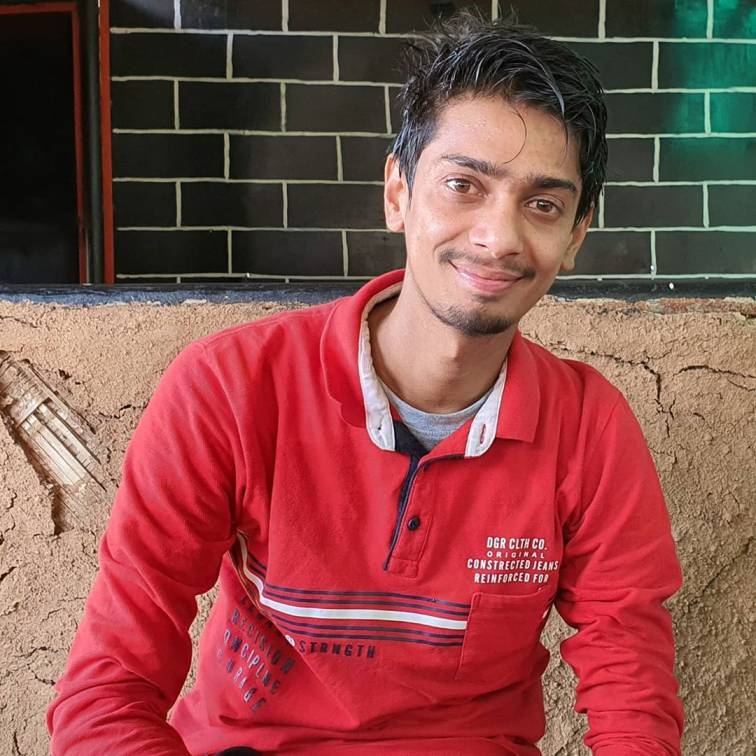
\includegraphics[width = 0.65\textwidth]{images/dimpu.jpg}
    \caption{Cultural Icon}
    \label{fig:dimpu}
\end{figure}
See Assamese cultural icon here \ref{fig:dimpu}.\cite{ismail2017identification}  He speaks a distinctive dialect. The claim has however been dismissed by some experts. \cite{glob}

\section{Equation}
    $ 2 \int_{10}^{13} x dx = y $
    $$ x=2 $$
\begin{equation}
    x^2 - 5x + 6 = \frac{p}{e^{-x} + \sin{x}}
\end{equation}
\begin{equation}
    \sum_{i=1}^{\infty} x^2 = \mu
\end{equation}

\begin{equation}
    |x| = \begin{cases}
            x & \text{ if } x \geq 0 \\
            -x & \text{ if } x < 0 \\
          \end{cases}
\end{equation}

\section {Bibliography}
This article was referred to. \cite{sarma2009some}

\printbibliography

\end{document}
